\documentclass[a4paper,12pt]{article}
%\documentclass[a4paper,10pt]{scrartcl}

\usepackage[utf8x]{inputenc}
\usepackage{amsfonts}
\usepackage{amsmath,esint}
\usepackage{graphicx}
\usepackage{pdfpages}
\usepackage{sansmath}
\usepackage{hyperref}
\usepackage{natbib}
\usepackage{caption}

\usepackage{tikz}


\definecolor{boiseBlue} {RGB}{29,72,159}
\definecolor{rojoAmor} {RGB}{171,13,4}
\definecolor{moradoAmor} {RGB}{93,8,113}
\definecolor{verdeAmor} {RGB}{98,158,31}
\definecolor{negro} {RGB}{10,10,10}
\definecolor{lgreen} {RGB}{180,210,100}
\definecolor{dblue}  {RGB}{20,66,129}
\definecolor{ddblue} {RGB}{11,36,69}
\definecolor{lred}   {RGB}{220,0,0}
\definecolor{nred}   {RGB}{224,0,0}
\definecolor{norange}{RGB}{230,120,20}
\definecolor{nyellow}{RGB}{255,221,0}
\definecolor{ngreen} {RGB}{98,158,31}
\definecolor{dgreen} {RGB}{78,138,21}
\definecolor{nblue}  {RGB}{28,130,185}
\definecolor{jblue}  {RGB}{20,50,100}

\usepackage{listings}
\usepackage{xcolor}
\usepackage{verbatim}
\lstset{language=C++,
		basicstyle=\ttfamily,
	       backgroundcolor=\color{black!5}\ttfamily,
                keywordstyle=\color{nblue}\ttfamily,
                stringstyle=\color{nred}\ttfamily,
                commentstyle=\color{ngreen}\ttfamily,
                morecomment=[l][\color{moradoAmor}]{\#}
}

\newenvironment{rcases}{\left.\begin{aligned}}{\end{aligned}\right\rbrace}

\renewcommand{\familydefault}{\sfdefault}

\newcommand{\specialcell}[2][c]{%
  \begin{tabular}[#1]{@{}c@{}}#2\end{tabular}}
% \specialcell{Foo\\bar}

\title{Wave interferometry\\{\normalsize Diego Domenzain}}
\author{}
\date{}

\pdfinfo{%
  /Title    ()
  /Author   ()
  /Creator  ()
  /Producer ()
  /Subject  ()
  /Keywords ()
}

\begin{document}
\maketitle
%-------------------
% main flow
%-------------------
\section*{Interferometry assumptions and goals}
In this setting {\it interferometry} we will refer to the processing technique whose input is a known energy response at receiver locations (observed data) and its output is a re-arranged energy response as if one of the receivers acted as a source.
\\\\
{\it Interferometry} exploits source-receiver reciprocity and the governing equations of the energy transfer in consideration by means of either cross-correlation (CI) or de-convolution (DI) of the observed data. Assumptions on the media of propagation will differ from which method is used. The propagating media and the energy transfer will dictate the required geometry of the sources for the input data.
\\\\
In a general setting, interferometry is useful (up to approximations of the method) for two things: 
\begin{enumerate}
\item retrieving a source-receiver field from passive observed data where the real source locations and/or time durations are unknown,
\item generating new source-receiver fields from active observed data where the real source locations and durations are known.
\end{enumerate}
%
\vspace{0.5em}
In the following, let $\partial\Omega_s$ be a surface where sources $s$ lie, and $\partial\Omega_r$ be a surface where receivers $r$ lie. Symbol $*$ denotes convolution, letters $a,b,c,r$ will denote receivers, $s$ sources and $u(b\gets s,t)$ will denote the wavefield $u$ at time $t$ observed at $b$ with source $s$.
%-------------------
% xcorr
%-------------------
\section*{Interferometry by cross-correlation}
\begin{align}
u(b\gets a,t) &= \int_{\partial\Omega_s} u(b\color{moradoAmor}\gets\color{black}s,t)*u(a\color{boiseBlue}\gets\color{black}s,-t)\,{\rm d}s.
\label{eqn:ci}
\end{align}
\subsection*{Discretization of CI}
Let $b_s$ denote the $n_{t}\times 1$ vector whose entries are the amplitude in time $t$ of a wavefield with source at $s$ and observed at $b$, $B_s$ denote an $n_{t}\times n_b$ matrix whose columns are $b_s$ for varying $b$ and fixed $s$, and $\star$ denote the column-wise crosscorrelation operation. In practice we compute equation \ref{eqn:ci} for many receivers $b$, 
\begin{align}
B_a = \sum_s B_s \star a_s.
\end{align}
Matrix $B_a$ has size $n_{2t-1}\times n_b$ and is called the {\it virtual shot-gather} with source at receiver $a$.
%-------------------
% decon
%-------------------
\section*{Interferometry by deconvolution}
\begin{align}
u(b\color{moradoAmor}\gets\color{black}s,t) &= \int_{\partial\Omega_r} u(b\gets a,t)*u(a\color{boiseBlue}\gets\color{black}s,t)\,{\rm d}r_a
\label{eqn:di}
\end{align}
In practice we have to go one step further to solve \ref{eqn:di},
\begin{align}
u(b\color{rojoAmor}\gets\color{black}c,t) &= \int_{\partial\Omega_r} u(b\gets a,t)*u(a\color{verdeAmor}\gets\color{black}c,t)\,{\rm d}r_a
\label{eqn:di-by-ci}
\end{align}
where,
\begin{align}
u(b\color{rojoAmor}\gets\color{black}c,t) &= \int_{\partial\Omega_s} u(b\color{moradoAmor}\gets \color{black}s,t)*u(c\color{nyellow}\gets\color{black}s,-t)\,{\rm d}s\\
u(a\color{verdeAmor}\gets\color{black}c,t) &= \int_{\partial\Omega_s} u(a\color{boiseBlue}\gets \color{black}s,t)*u(c\color{nyellow}\gets\color{black}s,-t)\,{\rm d}s
\label{eqn:di-by-ci-2}
\end{align}
\subsection*{Discretization of DI}
We discretize equation \ref{eqn:di-by-ci} in the frequency domain for a fixed frequency $\omega$ as, 
\begin{align}
\tilde{B}_C &= \tilde{B}_A \cdot \tilde{A}_C.
\label{eqn:di-d}
\end{align}
A column of $\tilde{B}_C$ is the wavefield in the frequency domain (with fixed $\omega$) from a source $c$ to receivers $b$ and it has size $n_b\times n_c$. A similar definition follows for matrices $\tilde{B}_A$ and $\tilde{A}_C$. A column of matrix $\tilde{B}_C$ (and similarly a column of $\tilde{A}_C$) is obtained by first computing $B_c$ for a given receiver $c$, transforming $B_c$ to the frequency domain, picking the row corresponding to the fixed $\omega$, and putting this row as a column in $\tilde{B}_C$ indexing it by $c$.
\\\\
Equation \ref{eqn:di-d} has to be solved for $\tilde{B}_A$ for as many time-frequencies we want our retrieved wavefield $B_a$ to have. Let $n_\omega$ be this number. After solving \ref{eqn:di-d} for $n_\omega$ times we arrange each $\tilde{B}_A$ (one for each $\omega$, $n_\omega$ such matricies) in the cube $\tilde{B}_{A\omega}$ of size $n_\omega\times n_b\times n_a$. This cube holds all virtual gathers $B_a$ for all virtual sources $a$ in the frequency domain as vertical planes fixing $a$.
\\\\
The full process for solving \ref{eqn:di} is,
\begin{align}
B_c &= \sum_s B_s \star c_s & \text{repeat for many $c$},\\
A_c &= \sum_s A_s \star c_s & \text{repeat for many $c$},\\
\tilde{B}_A &= \tilde{A}_C^{-1}\cdot \tilde{B}_C & \text{repeat for all $\omega$}.
\end{align}
\begin{figure}[!h]
\centering
% left low right up
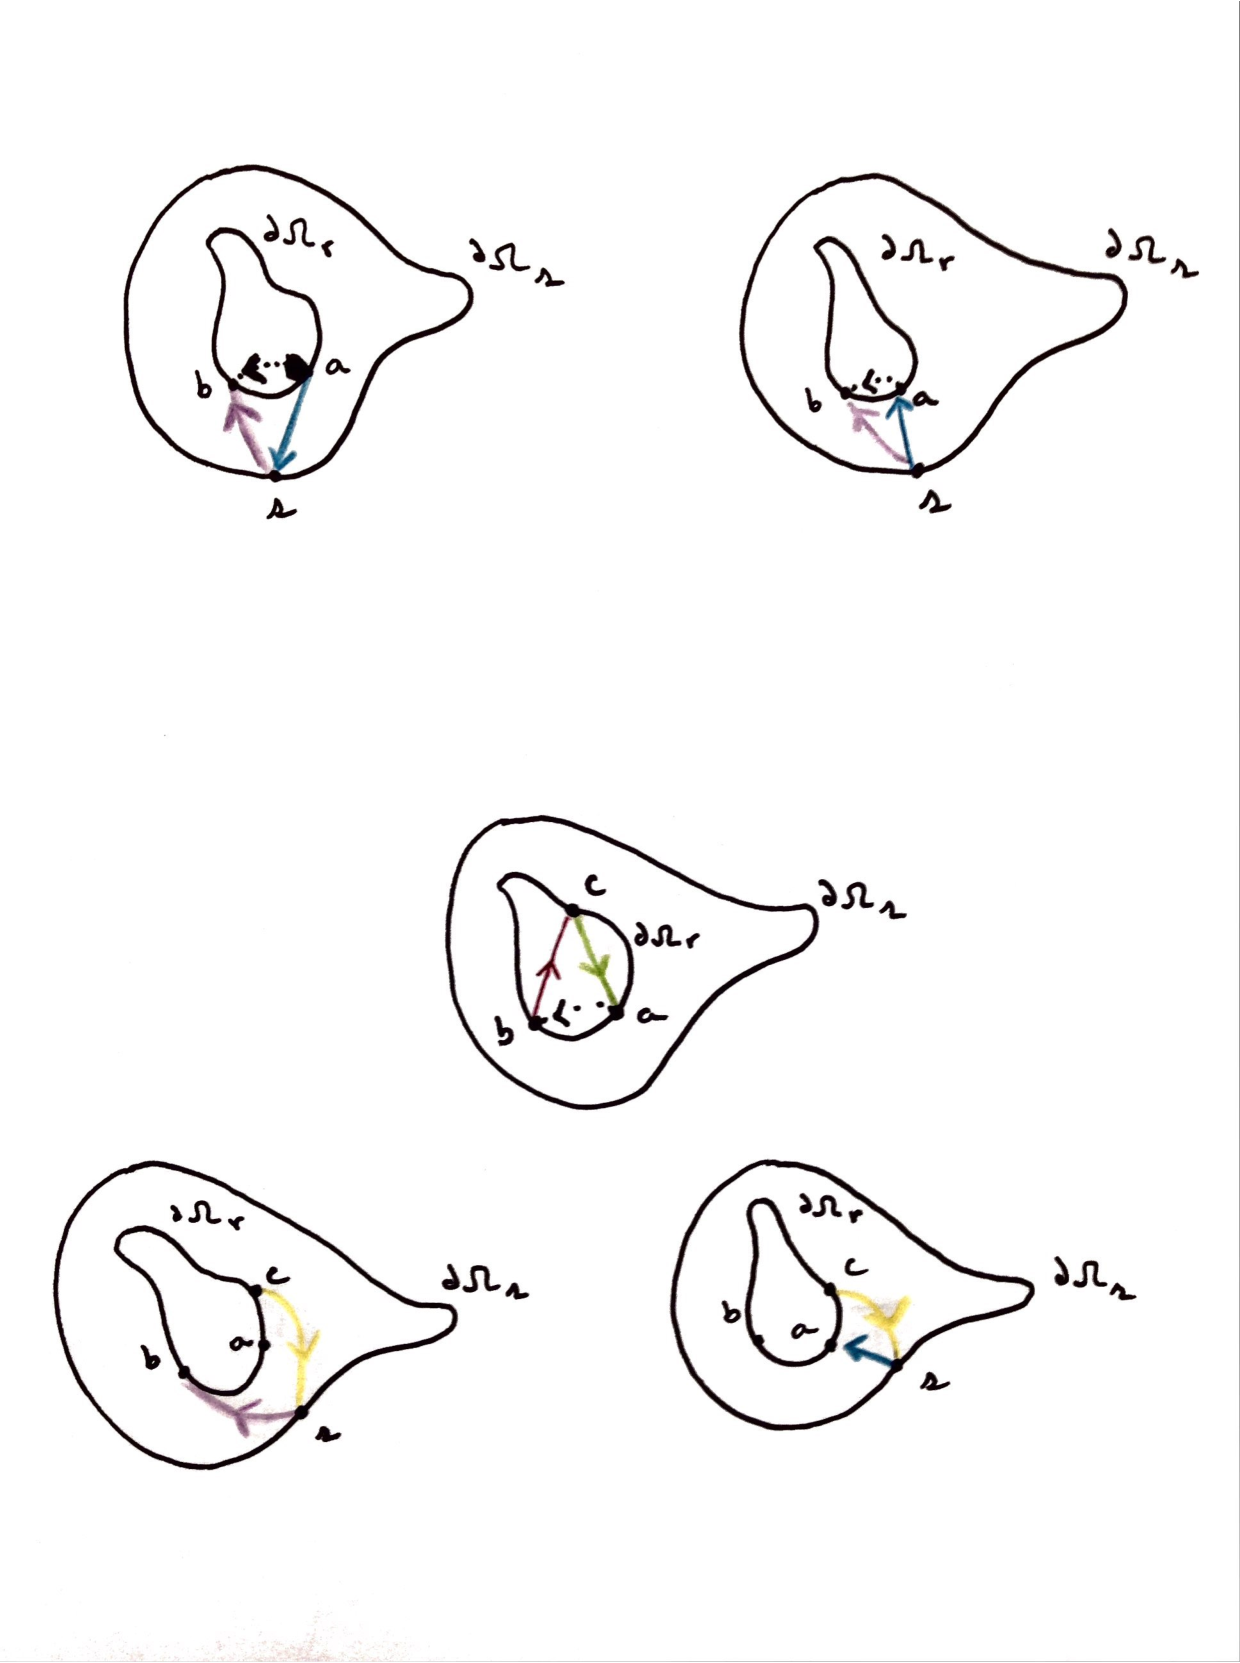
\includegraphics[trim={10 540 10 50},clip,width=1\textwidth]{../pics/interferometry-diagram.pdf}
\label{fig:ci-di}
\caption{Diagram of wavefields employed in interferometry by cross-correlation ({\it left}) and by deconvolution ({\it right}).}
\end{figure}
\begin{figure}[!h]
\centering
% left low right up
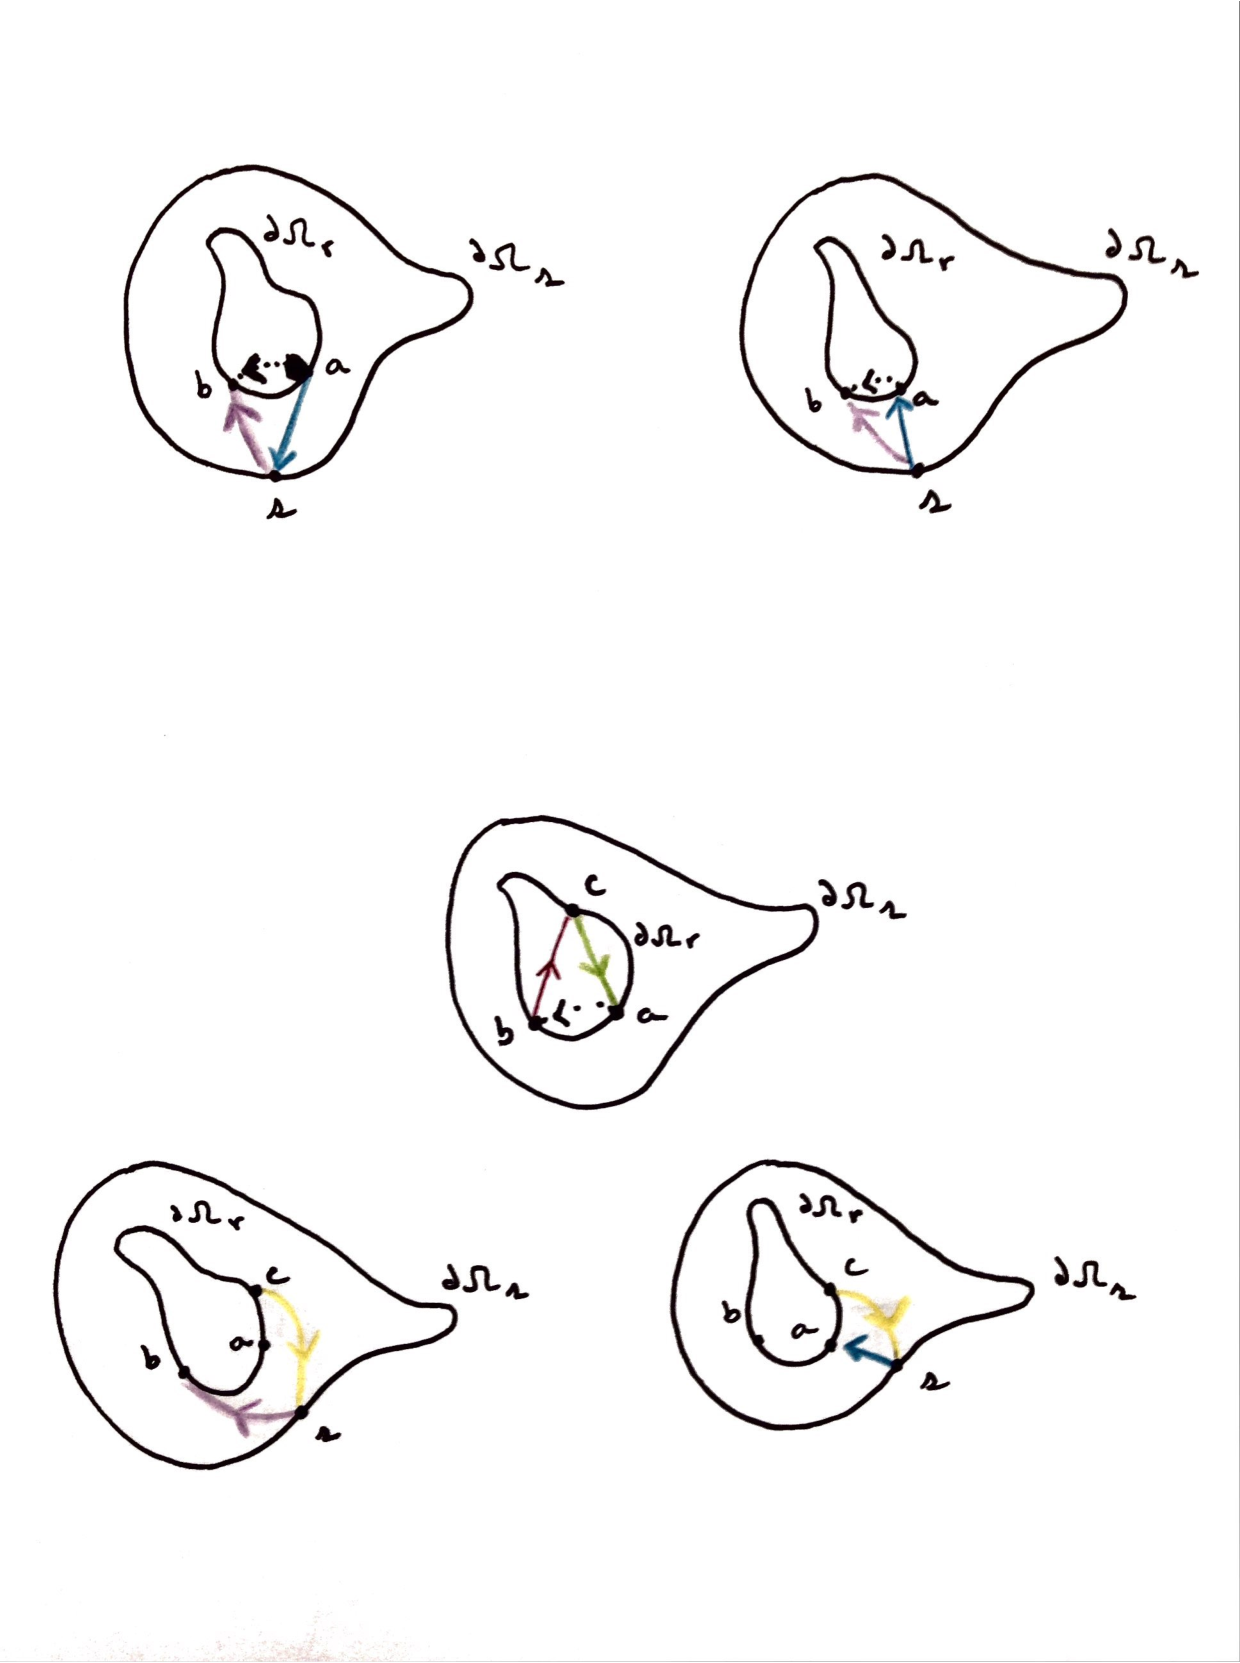
\includegraphics[trim={10 90 10 390},clip,width=0.8\textwidth]{../pics/interferometry-diagram.pdf}
%\label{fig:di-by-ci}
\caption{Diagram of wavefields employed in interferometry by deconvolution using interferometry by cross-correlation.}
\end{figure}
%-------------------
% decon by xcorr
%-------------------
\clearpage
\section*{DI by CI}
\begin{align}
u(b\color{rojoAmor}\gets\color{black}c,t) &= \int_{\partial\Omega_r} u(b\gets a,t)*u(a\color{verdeAmor}\gets\color{black}c,t)\,{\rm d}r_a
%\label{eqn:di-by-ci}
\end{align}
where,
\begin{align}
u(b\color{rojoAmor}\gets\color{black}c,t) &= \int_{\partial\Omega_s} u(b\color{moradoAmor}\gets \color{black}s,t)*u(c\color{nyellow}\gets\color{black}s,-t)\,{\rm d}s\\
u(a\color{verdeAmor}\gets\color{black}c,t) &= \int_{\partial\Omega_s} u(a\color{boiseBlue}\gets \color{black}s,t)*u(c\color{nyellow}\gets\color{black}s,-t)\,{\rm d}s
%\label{eqn:di-by-ci-2}
\end{align}
\subsection*{Discretization of DI by CI}
\begin{align}
B_c &= \sum_s B_s \star c_s & \text{repeat for many $c$},\\
A_c &= \sum_s A_s \star c_s & \text{repeat for many $c$},\\
\tilde{B}_A &= \tilde{A}_C^{-1}\cdot \tilde{B}_C & \text{repeat for all $\omega$}.
\end{align}
\begin{figure}[!h]
\centering
% left low right up
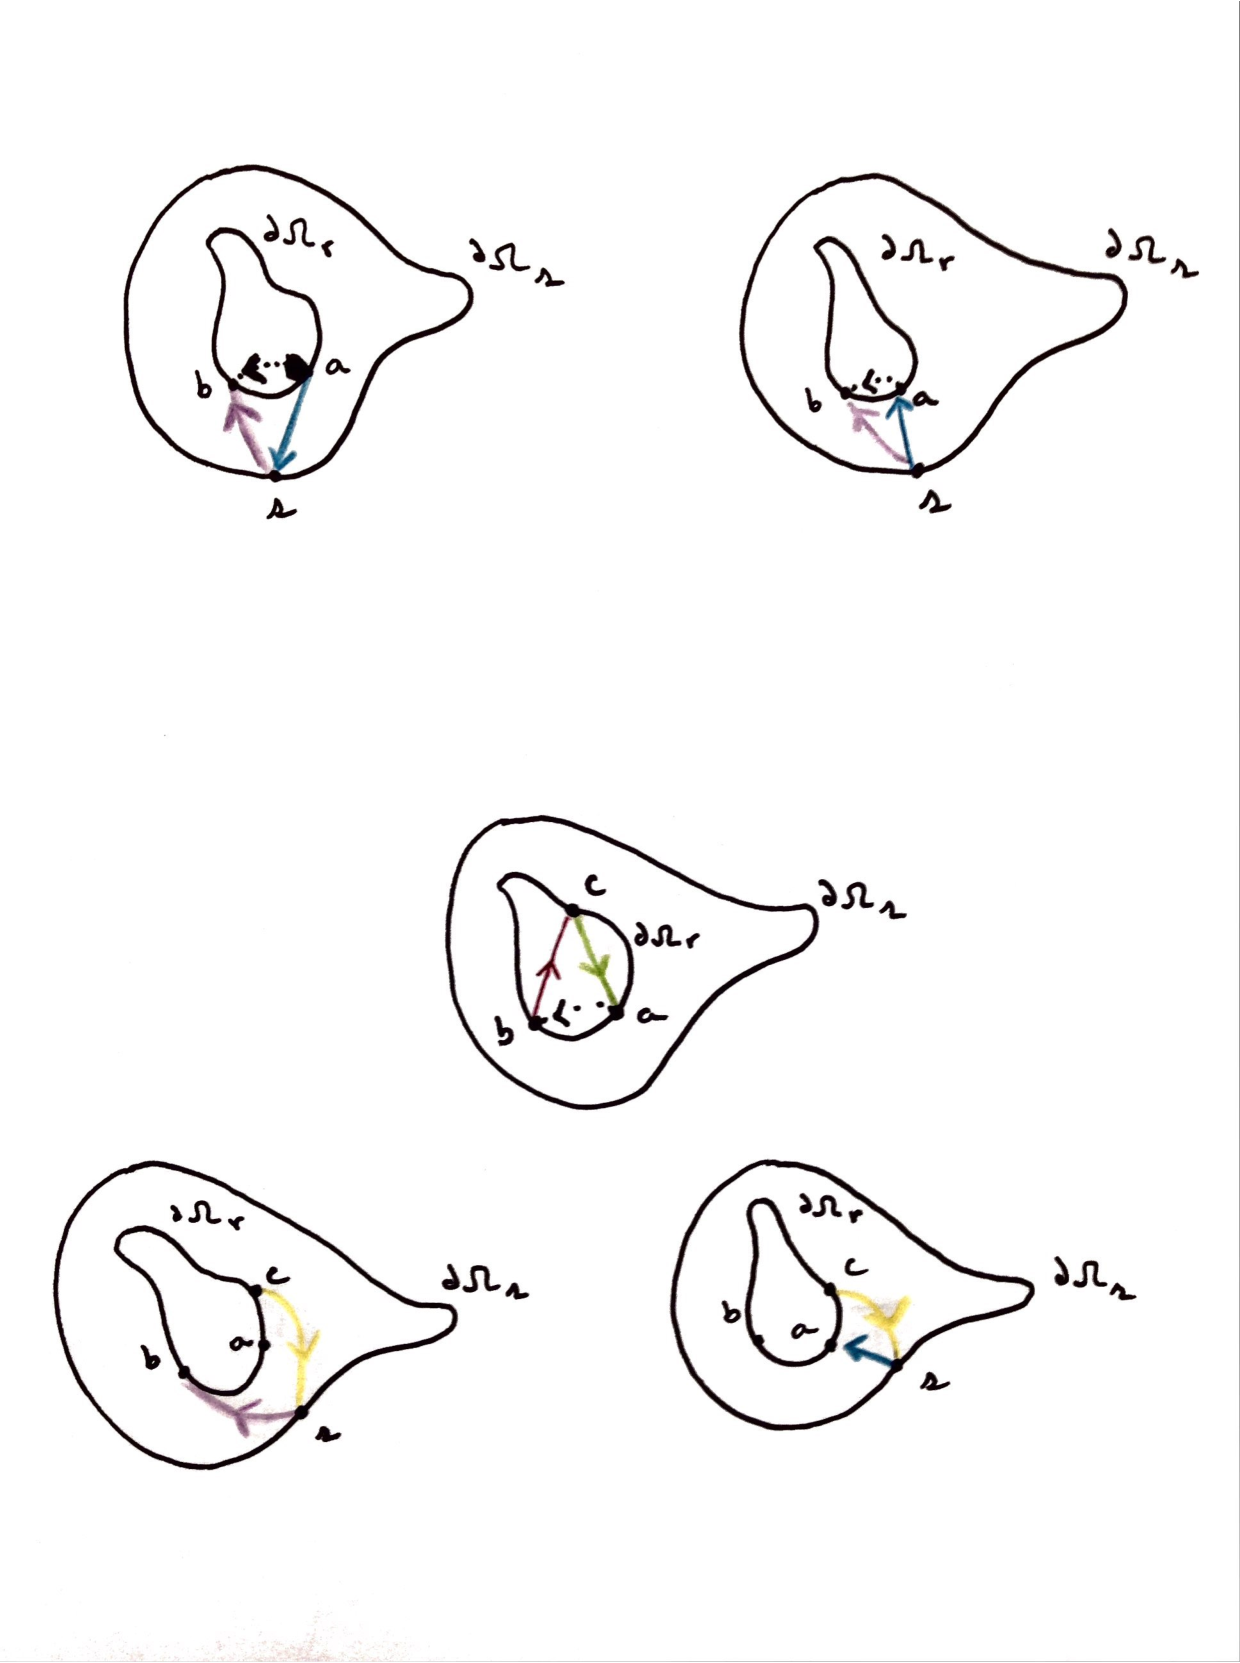
\includegraphics[trim={10 90 10 390},clip,width=0.8\textwidth]{../pics/interferometry-diagram.pdf}
%\label{fig:di-by-ci}
\caption{Diagram of wavefields employed in interferometry by deconvolution using interferometry by cross-correlation.}
\end{figure}
%
%
%------------
% biblio
%------------
%\newpage
\bibliographystyle{plainnat}
\bibliography{interferometry-theory}
%\nocite{*}
\end{document}